% Self-contained CVaR diagram — compile with: pdflatex cvar.tex
% Output: cvar.pdf (single tightly-cropped page).
\documentclass[border=10pt]{standalone}
\usepackage{tikz}
\usepackage{amsmath, amssymb}
\usepackage{xcolor}

% --- Font-size compensation for down-scaled inclusion --------------------
% This diagram is included in the paper at a fraction of its natural width
% (see sec-design.tex), which shrinks every label. \small and \scriptsize are
% redefined here so that labels land near 8pt and tick marks near 6.5pt in the
% typeset paper. Re-tune if the \includegraphics width changes.
\usepackage{anyfontsize}
\renewcommand{\small}{\fontsize{19.3}{23.2}\selectfont}
\renewcommand{\scriptsize}{\fontsize{15.7}{18.8}\selectfont}
\usetikzlibrary{patterns}

% Palette (subdued, paper-style)
\definecolor{cInk}{HTML}{222222}
\definecolor{cMute}{HTML}{777777}
\definecolor{cAccent2}{HTML}{B23A48}
\definecolor{cAccent2Soft}{HTML}{F0CCD0}

\begin{document}
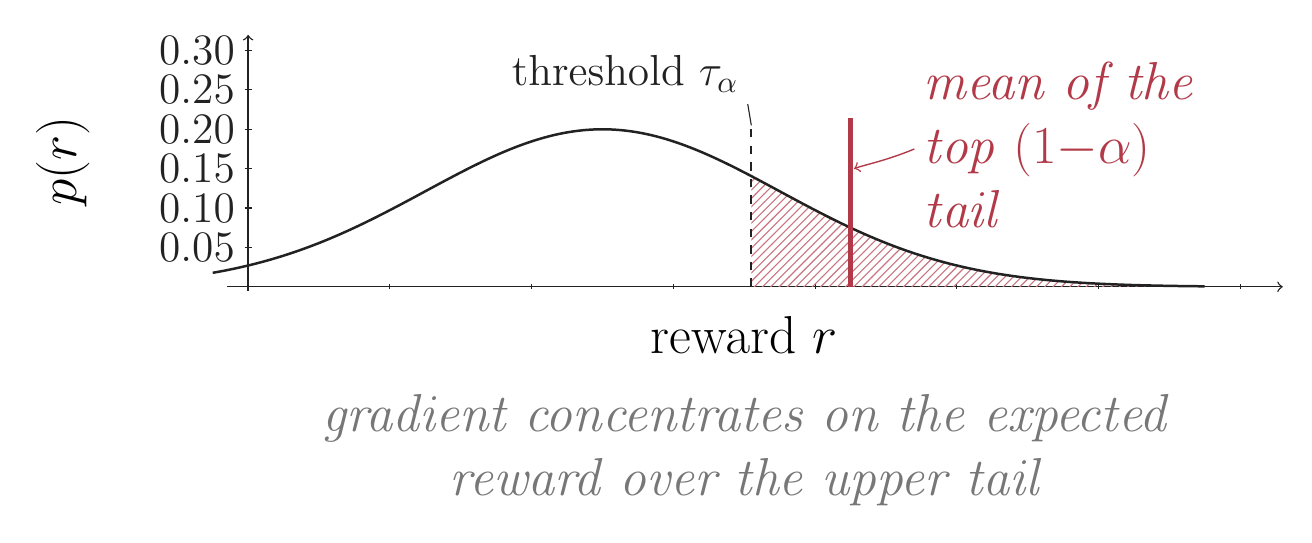
\begin{tikzpicture}[x=0.9cm, y=10cm]

  % Plot frame: x = reward in [-4, 10], y = density in [0, 0.32]
  % Reward distribution: N(mu=1, sigma=2.5), peak amp 0.20.
  %   tau-quantile (tau=0.8):  Q_0.8 ~= 3.10
  %   CVaR_{1-tau}             ~= 4.50

  \draw[->, line width=0.5pt, color=cInk] (-4.3, 0)    -- (10.6, 0);
  \draw[->, line width=0.5pt, color=cInk] (-4.0,-0.005) -- (-4.0, 0.32);
  \node[font=\small, anchor=north] at (3.0, -0.025) {reward $r$};
  \node[font=\small, rotate=90, anchor=south] at (-6.10, 0.16) {$p(r)$};

  \foreach \y/\lab in {0.05/0.05, 0.10/0.10, 0.15/0.15, 0.20/0.20, 0.25/0.25, 0.30/0.30}{
    \draw[line width=0.4pt, color=cInk] (-4.05,\y) -- (-3.95,\y);
    \node[font=\scriptsize, color=cInk, anchor=east, xshift=-0.05cm] at (-4.0,\y) {\lab};
  }
  \foreach \x in {-4,-2,0,2,4,6,8,10}{
    \draw[line width=0.4pt, color=cInk] (\x,-0.003) -- (\x, 0.003);
  }

  % Shaded right tail beyond Q_0.8 ~= 3.1
  \begin{scope}
    \clip (3.10, 0) rectangle (9.0, 0.32);
    \fill[cAccent2Soft, pattern=north east lines, pattern color=cAccent2!70,
          smooth, samples=200, domain=3.10:9.0]
          plot (\x, {0.20 * exp(-0.5*((\x-1.0)/2.5)^2)})
          -- (9.0, 0) -- (3.10, 0) -- cycle;
  \end{scope}

  % Reward density curve
  \draw[line width=0.9pt, color=cInk, smooth, samples=240, domain=-4.5:9.5]
        plot (\x, {0.20 * exp(-0.5*((\x-1.0)/2.5)^2)});

  % Quantile threshold (dashed)
  \draw[dashed, line width=0.7pt, color=cInk] (3.10, 0) -- (3.10, 0.20);
  \node[font=\scriptsize, color=cInk, anchor=south east] at (3.05, 0.235)
        {threshold $\tau_\alpha$};
  \draw[line width=0.4pt, color=cInk] (3.05, 0.232) -- (3.10, 0.205);

  % CVaR = mean of right tail (solid bold red bar)
  \draw[line width=1.6pt, color=cAccent2] (4.50, 0) -- (4.50, 0.215);

  \node[font=\small\itshape, color=cAccent2, anchor=west, align=left] at (5.4, 0.18)
        {mean of the\\top $(1{-}\alpha)$\\tail};
  \draw[->, line width=0.5pt, color=cAccent2] (5.4, 0.175) .. controls
        (5.0, 0.16) and (4.7, 0.155) .. (4.55, 0.150);

  \node[font=\small\itshape, color=cMute, anchor=north, align=center] at (3.0, -0.125)
        {gradient concentrates on the expected\\reward over the upper tail};

\end{tikzpicture}
\end{document}
